
\chapter{Telas da Aplicação}
\label{chap:telas}

A figura \ref{img:tela_de_login} mostra a tela de login da aplicação. O login pode ser feito via Facebook, Google ou criando uma conta local.

\begin{figure}[H]
    \centering
    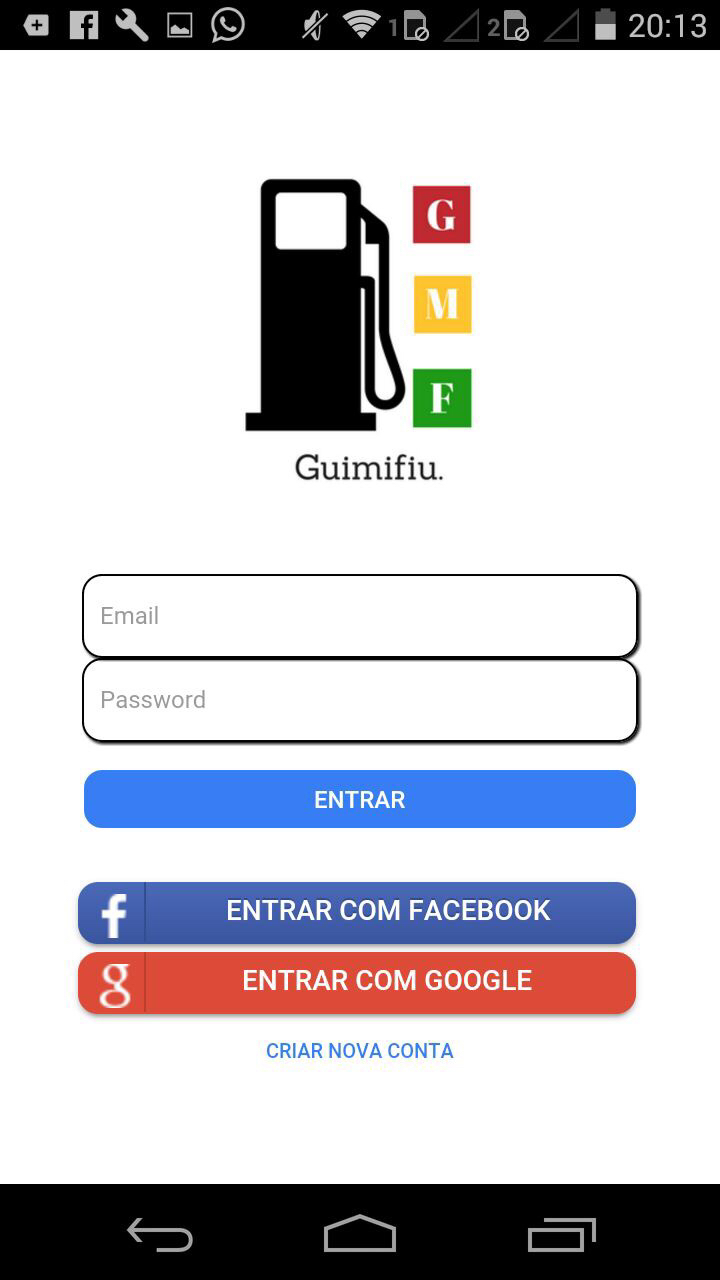
\includegraphics[scale=0.5]{figuras/app_1.jpg}
    \caption[Tela de login]{Tela de login. Fonte: autores}
    \label{img:tela_de_login}
\end{figure}

Como ilustrado na figura \ref{img:postos_de_gasolina_proximos}, são mostrados na aplicação todos os postos de combustíveis próximos a localização do usuário em um raio de 5km.

\begin{figure}[H]
    \centering
    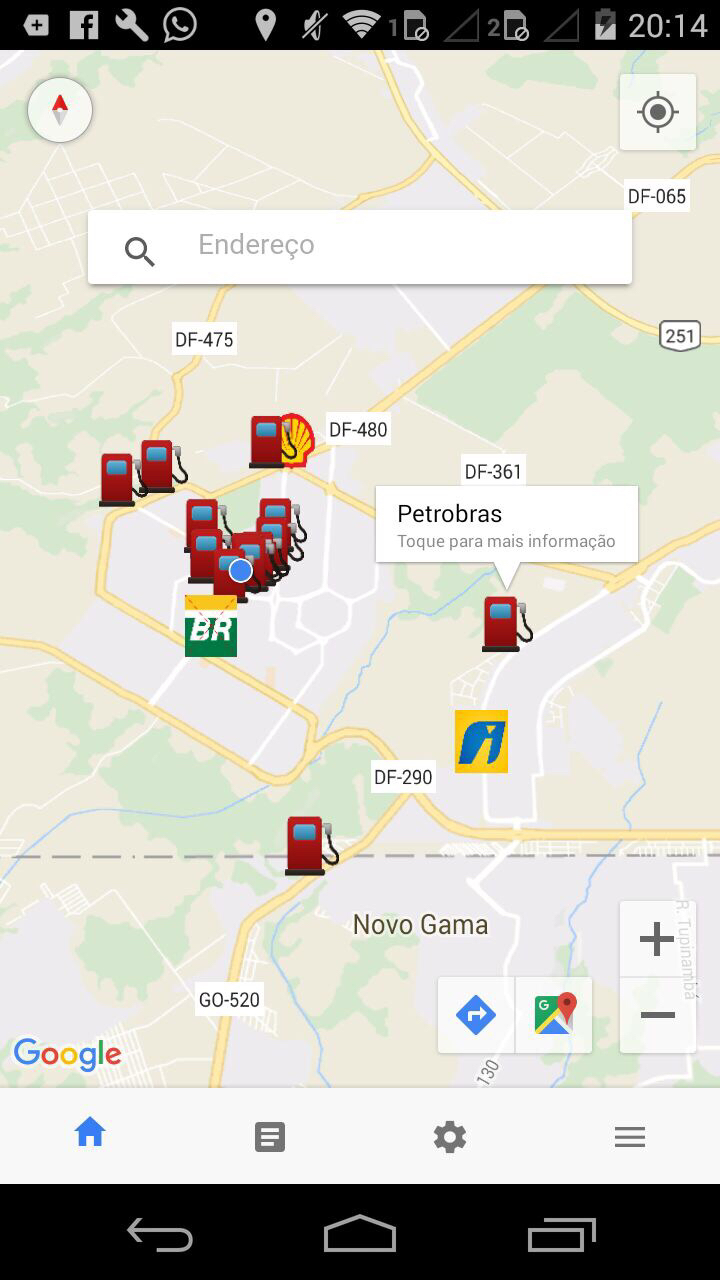
\includegraphics[scale=0.5]{figuras/app_2.jpg}
    \caption[Postos de combustíveis próximos]{Postos de combustíveis próximos. Fonte: autores}
    \label{img:postos_de_gasolina_proximos}
\end{figure}

É possível também inserir um endereço para o aplicativo planejar uma rota e mostrar todos os postos de combustíveis perto daquela rota, como ilustram as figuras \ref{img:buscando_localizacoes}, \ref{img:localizacao_encontrada} e \ref{img:postos_de_gasolina_proximos_em_uma_rota}.

\begin{figure}[H]
    \centering
    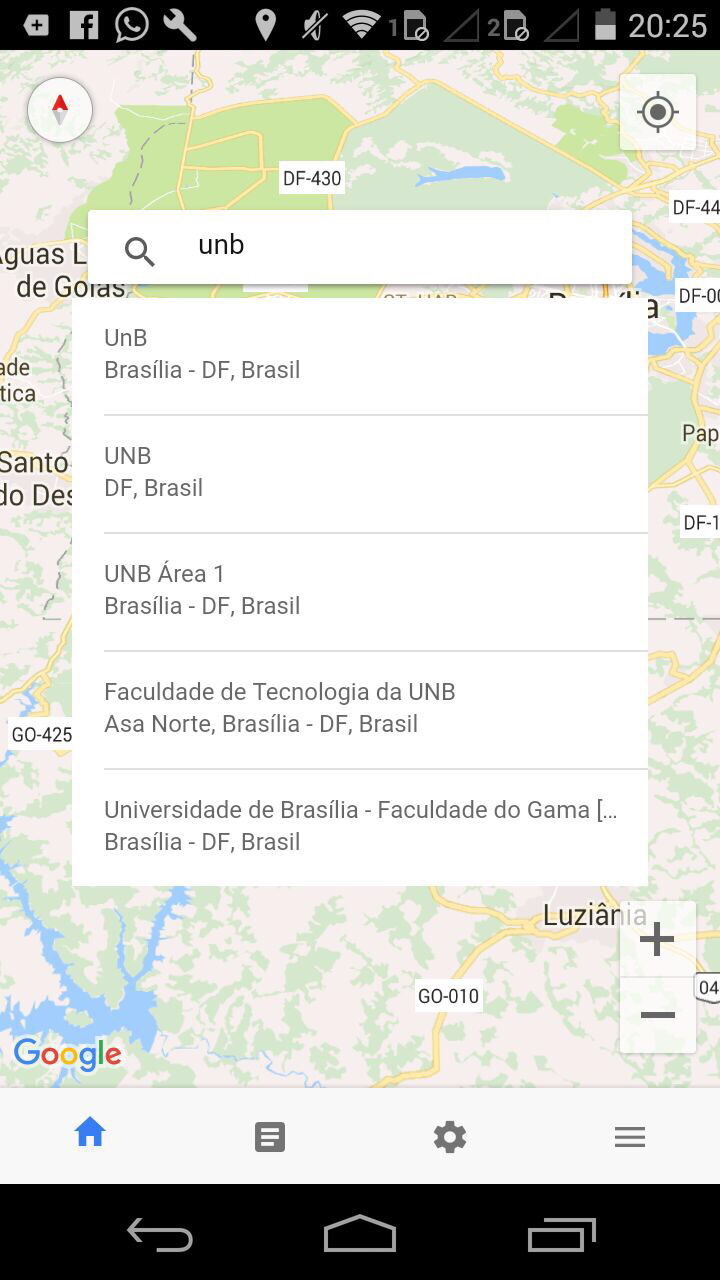
\includegraphics[scale=0.5]{figuras/app_3.jpg}
    \caption[Buscando localizações]{Buscando localizações. Fonte: autores}
    \label{img:buscando_localizacoes}
\end{figure}

\begin{figure}[H]
    \centering
    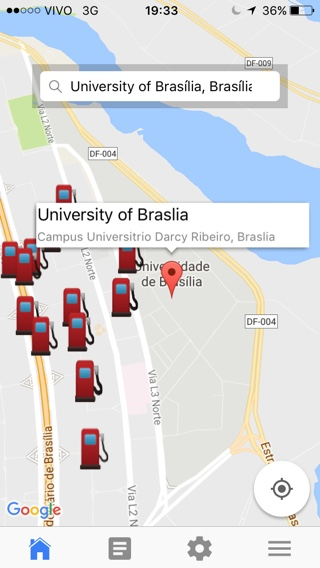
\includegraphics[scale=0.5]{figuras/app_4.jpg}
    \caption[Localização encontrada]{Localização encontrada. Fonte: autores}
    \label{img:localizacao_encontrada}
\end{figure}

\begin{figure}[H]
    \centering.
    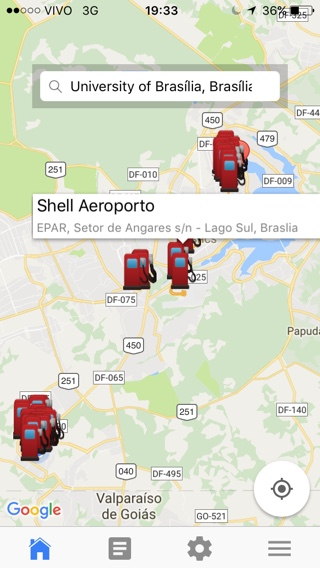
\includegraphics[scale=0.5]{figuras/app_5.jpg}
    \caption[Postos de combustíveis próximos em uma rota]{Postos de combustíveis próximos em uma rota. Fonte: autores}
    \label{img:postos_de_gasolina_proximos_em_uma_rota}
\end{figure}
